\documentclass[thesis=M,english]{FITthesis}[2012/06/26]

\usepackage[utf8]{inputenc}
\usepackage[T1]{fontenc}

\usepackage{graphicx}
\usepackage{tabularx}
\usepackage{booktabs}
\usepackage{csvsimple}
\usepackage{rotating}
\usepackage{subcaption}
\usepackage[usenames,dvipsnames]{xcolor}
\usepackage{blindtext}
\usepackage{dirtree}
\usepackage{pifont}
\usepackage{amsfonts}
\usepackage{tikz}
\usepackage{minted}


\newcommand{\myblindtext}{\textcolor{Gray}{\blindtext}}
\newcommand{\myBlindtext}{\textcolor{Gray}{\Blindtext}}
\newcommand{\todo}[1]{\textcolor{red}{[[#1]]}}
\newcommand{\edit}[1]{\textcolor{blue}{#1}}
\newcommand{\yesMark}{\textcolor{Green}{\ding{51}}}
\newcommand{\noMark}{\textcolor{red}{\ding{55}}}
\newcommand{\nodewidth}{2.5cm}
\newcommand{\nodeheight}{0.6cm}

\usemintedstyle{bw}
\setminted{frame=lines,linenos,fontsize=\footnotesize,breaklines}

\newcommand{\yesbf}[1]{
  \ifthenelse{\equal{#1}{yes}}{\textbf{#1}}{#1}
}
\newcommand{\csvtable}[3]{
  \toprule
  #2 \\
  \midrule
  \csvreader[separator=semicolon,late after line=\\]{#1}{}{#3}
  \bottomrule
}

\usetikzlibrary{arrows.meta,calc,decorations.pathreplacing,fit,matrix,positioning}
\pgfdeclarelayer{bg}
\pgfsetlayers{bg,main}
\definecolor{orange}{RGB}{255,204,0} % #ffcc00
\tikzset{
  >=stealth,
  font=\footnotesize,
  node distance=\nodeheight,
  rect/.style={draw,fill=orange,shape=rectangle,minimum width=\nodewidth,minimum height=\nodeheight,inner sep=1mm,text height=1.5ex,text depth=0.25ex},
  smallrect/.style={rect,minimum width=0.5*\nodewidth},
  circle/.style={draw,fill=orange,shape=circle,minimum size=\nodeheight,inner sep=0},
  line/.style={draw,->,very thick,rounded corners},
  struct/.style={matrix,inner sep=0,column sep=-\pgflinewidth},
  xor/.style={inner sep=0}
}




\department{Department of Computer Systems}
\title{Current Development of Authenticated Encryption and its Usage in the TLS Protocol}
\authorGN{Jan}
\authorFN{Žák}
\authorWithDegrees{Bc. Jan Žák}
\supervisor{prof. Ing. Róbert Lórencz, CSc.}
\acknowledgements{My sincere thanks goes to prof. Wu Hongjun, Assistant Professor at Nangyang Technological University, Singapore, who served as my external supervisor, advised about my thesis and provided an invaluable insight into the field of authenticated encryption.}
\abstractEN{This thesis focuses on adding a new authenticated encryption cipher suite in the OpenSSL implementation of the TLS protocol using the EVP API. The cipher was selected from CAESAR competition submissions. The new cipher suite was successfully tested by analysing TLS network communication between server and client.}
\abstractCS{Tato práce se zaměřuje na přidání nové šifrovací sady s autentizovaným šifrováním do OpenSSL implementace TLS protokolu použitím EVP API. Nová šifra byla vybrána z přihlášených algoritmů do CAESAR soutěže. Nová šifrovací sada byla úspěšně otestována analýzou TLS síťové komunikace mezi serverem a klientem.}
\placeForDeclarationOfAuthenticity{Prague}
\declarationOfAuthenticityOption{4}
\keywordsCS{autentizované šifrování s přidruženými daty,caesar soutěž,openssl evp api,openssl knihovna,tls šifrovací sady,tls protokol}
\keywordsEN{authenticated encryption with associated data,caesar competition,openssl evp api,openssl library,tls cipher suite,tls protocol}


\begin{document}


\begin{introduction}

At its core, the Internet is built on top of IP and TCP protocols, which are used to package data into small packets for transport. As these packets travel across the world, they cross many computer systems in many countries. Because the core protocols do not provide any security by themselves, anyone with access to the communication links can gain full access to the data as well as change the traffic without detection.

Over the last years, the Internet has grown into a major platform for the world's communication. The Internet's trustworthiness has become critical to its success. If a person cannot trust that they are communicating with the party they intend, they will not give out their confidential data. If they cannot be assured that delivered information is not modified in transit, they will not trust it as much.

Currently the TLS protocol uses a MAC-then-Encrypt generic composition of encryption and authentication algorithm to achieve both confidentiality and integrity. More recently, the idea of using a single cryptosystem has become accepted. In this concept, the MtE composition is replaced by a single authenticated encryption algorithm, such as AES-GCM.

This thesis focuses on the OpenSSL cryptographic library, which is the most frequently used implementation of the TLS protocol worldwide. It implements a new authenticated encryption algorithm into the TLS protocol.

\end{introduction}

\chapter{Establishing secure communication channel}

\section{Encryption}

Encryption is the original goal of cryptography. It is the process of encoding messages in such a way that only authorized parties can read it. Encryption does not of itself prevent interception, but denies the message content to the interceptor.

The generic use case is: Alice and Bob\footnote{Alice, Bob and Eve are placeholder names commonly used when discussing cryptography, to identify an archetypal role of participant. Alice is a sender, Bob is a receiver and Eve is an eavesdropper. For the first time these names were used in Ron Rivest's paper introducing RSA public key cryptosystem \todo{Ref it}. Since then, a number of other names have entered cryptographic literature.} want to communicate with each other. However, communication channels are assumed not to be secure. Eve is eavesdropping on the channel. Any message that Alice sends to Bob is also received by Eve. (The same applies for messages sent from Bob to Alice, but it is the same problem and the same solution will work for Bob's messages, so we concentrate to Alice messages.) How can Alice and Bob communicate without learning everything? (\autoref{img:encryption_problem}) \cite[p.~23]{ferguson2010cryptography}

To prevent Eve from understanding the conversation, Alice and Bob are using encryption (\autoref{img:encryption}). They first agree on a cipher and a secret key. The secret key needs to be exchanged via some secure communication channel that Eve cannon eavesdrop on. Alice and Bob can meet in person to exchange the key, or Alice can mail it via public post service.

\begin{figure}
  \centering
  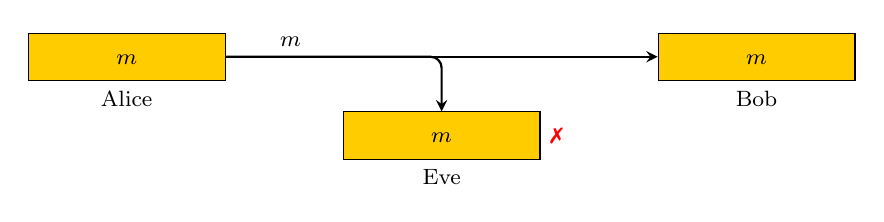
\begin{tikzpicture}
    \node (alice) at (0,0) [rect,label=below:{Alice}] {$m$};
    \node (bob) at (8,0) [rect,label=below:{Bob}] {$m$};
    \node (eve) at (4,-1) [rect,label=below:{Eve},label=right:{\noMark}] {$m$};
    \coordinate (channel) at (4,0);
    \draw [->,thick] (alice) -- (bob) node[pos=0.15,above]{$m$};
    \draw [->,thick,rounded corners] (alice) -- (channel) -- (eve);
  \end{tikzpicture}
  \caption{How can Alice and Bob communicate securely?}
  \label{img:encryption_problem}
\end{figure}

\begin{figure}
  \centering
  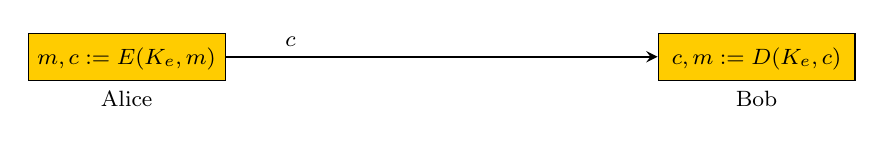
\begin{tikzpicture}
    \node (alice) at (0,0) [rect,label=below:{Alice}] {$m, c := E(K_e, m)$};
    \node (bob) at (8,0) [rect,label=below:{Bob}] {$c, m := D(K_e, c)$};
    \draw [->,thick] (alice) -- (bob) node[pos=0.15,above]{$c$};
  \end{tikzpicture}
  \caption{Generic setting for encryption}
  \label{img:encryption}
\end{figure}

\begin{figure}
  \centering
  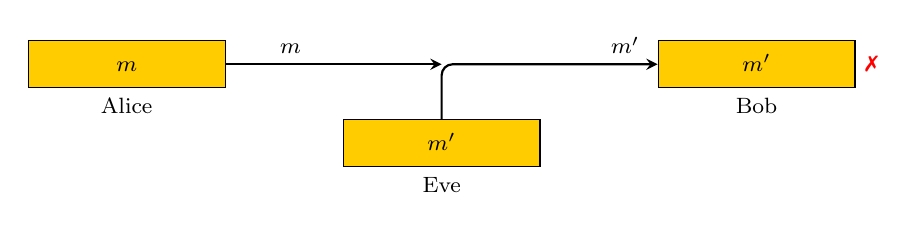
\begin{tikzpicture}
    \node (alice) at (0,0) [rect,label=below:{Alice}] {$m$};
    \node (bob) at (8,0) [rect,label=below:{Bob},label=right:{\noMark}] {$m'$};
    \node (eve) at (4,-1) [rect,label=below:{Eve}] {$m'$};
    \coordinate (channel) at (4,0);
    \draw [->,thick] (alice) -- (channel) node[pos=0.3,above]{$m$};
    \draw [->,thick,rounded corners] (eve) -- (channel) -- (bob) node[pos=0.85,above]{$m'$};
  \end{tikzpicture}
  \caption{How does Bob know who sent the message?}
  \label{img:authentication_problem}
\end{figure}

\begin{figure}
  \centering
  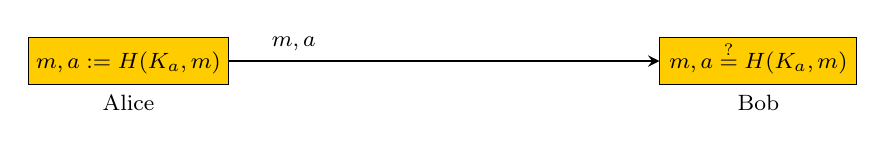
\begin{tikzpicture}
    \node (alice) at (0,0) [rect,label=below:{Alice}] {$m, a := H(K_a, m)$};
    \node (bob) at (8,0) [rect,label=below:{Bob}] {$m, a \stackrel{?}{=} H(K_a, m)$};
    \draw [->,thick] (alice) -- (bob) node[pos=0.15,above]{$m, a$};
  \end{tikzpicture}
  \caption{Generic setting for authentication}
  \label{img:authentication}
\end{figure}

\begin{figure}
  \centering
  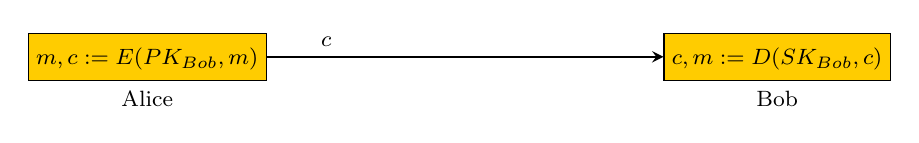
\begin{tikzpicture}
    \node (alice) at (0,0) [rect,label=below:{Alice}] {$m, c := E(PK_{Bob}, m)$};
    \node (bob) at (8,0) [rect,label=below:{Bob}] {$c, m := D(SK_{Bob}, c)$};
    \draw [->,thick] (alice) -- (bob) node[pos=0.15,above]{$c$};
  \end{tikzpicture}
  \caption{Generic setting for public-key encryption}
  \label{img:authentication}
\end{figure}

\begin{figure}
  \centering
  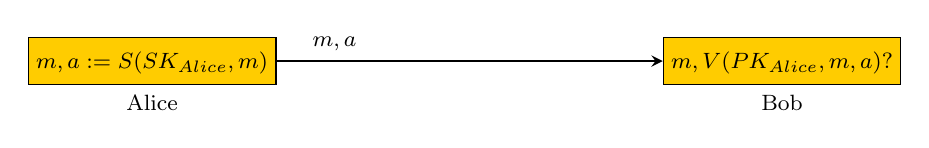
\begin{tikzpicture}
    \node (alice) at (0,0) [rect,label=below:{Alice}] {$m, a := S(SK_{Alice}, m)$};
    \node (bob) at (8,0) [rect,label=below:{Bob}] {$m, V(PK_{Alice}, m, a) ?$};
    \draw [->,thick] (alice) -- (bob) node[pos=0.15,above]{$m, a$};
  \end{tikzpicture}
  \caption{Generic setting for digital signature}
  \label{img:authentication}
\end{figure}


\chapter{Authenticated Encryption}

\todo{popis AEAD}

\section{Block cipher modes}

from 70s

\begin{description}
  \item[ECB]
  \item[CBC]
  \item[CFB]
  \item[OFB]
  \item[CTR]
\end{description}

\todo{Block cipher modes image from @angealbertini}

Exploiting malleability:

ECB: Rearrange, replay blocks
CTR, OFB: Bitwise modification of blocks
CBC: Change current ciphertext block to predictably change the next plaintext block (during decryption)

Chosen-boundary attacks:

ECB, CBC, CFB: Partial chosen-plaintext control
Decrypt messages byte by byte

Here come the XOR ninjas

\section{Authenticated Encryption}
\section{Authenticated Encryption with Associated Data}



\section{Generic compositions}

\begin{description}
  \item[Encrypt-and-MAC]
  \item[MAC-then-Encrypt]
  \item[Encrypt-then-MAC]
\end{description}

\begin{figure}
  \centering
  \begin{subfigure}[b]{0.3\textwidth}
    \centering
    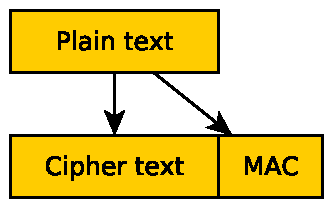
\includegraphics[width=0.9\textwidth]{images/encrypt-and-mac.pdf}
    \caption{Encrypt-and-MAC}
  \end{subfigure}
  \begin{subfigure}[b]{0.3\textwidth}
    \centering
    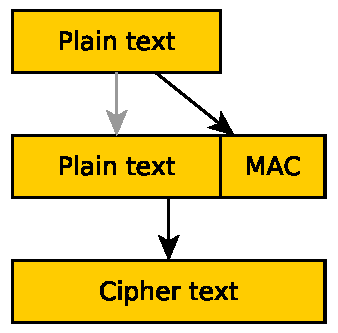
\includegraphics[width=0.9\textwidth]{images/mac-then-encrypt.pdf}
    \caption{MAC-then-encrypt}
  \end{subfigure}
  \begin{subfigure}[b]{0.3\textwidth}
    \centering
    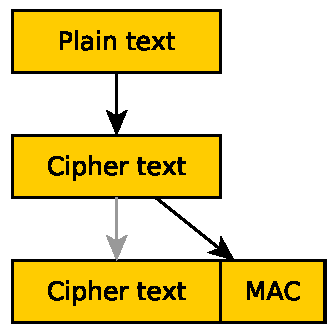
\includegraphics[width=0.9\textwidth]{images/encrypt-then-mac.pdf}
    \caption{Encrypt-then-MAC}
  \end{subfigure}
  \caption{Generic compositions of Authentized Encryption}
\end{figure}

\section{Competition for Authenticated Encryption: Security, Applicability and Robustness}

CAESAR is worldwide cryptographic competition, focused on finding new methods of authenticated encryption, that offer advantages against commonly used AES-GCM and will be suitable for widespread adoption. Submitted algorithms will be publicly evaluated by committee of researchers in fields of cryptography and cryptoanalysis.

\todo{popis algoritmů byly v soutěži, v čem se lišily, jaké a jak v nich byly nalezeny zranitelnosti a proto nepostoupily}

\todo{výběr algoritmu pro implementaci}

\subsection{Selection criteria}

\begin{description}
  \item[Online (one-pass)]
\end{description}



\input{text/aead-caesar-norx.tex}
\input{text/aead-caesar-selection.tex}



\chapter{Competition for Authenticated Encryption: Security, Applicability and Robustness}

In 2013, CAESAR was announced. It is a worldwide cryptographic competition, focused on finding new methods of authenticated encryption, that offer advantages against commonly used AES-GCM and will be suitable for widespread adoption. Submitted algorithms will be publicly evaluated by committee of researchers in fields of cryptography and cryptoanalysis.

This competition follows a long tradition of focused competitions in secret-key cryptography:

\begin{itemize}
  \item In 1997, United States National Institute of Standards and Technology (NIST) announced an open competition for a new symmetric cupher, Advanced Encryption Standard (AES). This competition attracted 15 submissions from 50 cryptographers around the world. In the end, Rijndael was chosen as AES.
  \item In 2004, European Network of Excellence in Cryptology (ECRYPT) announced the ECRYPT Stream Cipher Project (eSTREAM), a call for new stream ciphers suitable for widespread adoption. This call attracted 34 submissions from 100 cryptographers around the world. In the end, the eSTREAM committee selected a portfolio containing several stream ciphers.
  \item In 2007, NIST announced an open competition for a new hash standard to Secure Hash Algorithm family (SHA-3). This competition attracted 64 submissions from 200 cryptographers around the world. In the end, Keccak was chosen as SHA-3.
\end{itemize}

All past cryptographic competitions attracted many submissions from cryptographers around the world, and then even more security and performance evaluations from cryptanalysts. They are generally viewed as having provided a tremendous boost to the cryptographic research community's understanding of underlying concepts, and a tremendous increase in confidence in the security of some existing cryptosystems. Similar comments are expected to apply to CAESAR. \cite{crypto-competitions}


\section{Functional requirements}

For the purpose of CAESAR competition, an \textit{authenticated cipher} is a pair of encrypt and decrypt functions, meeting the following specific requirements.

All inputs and outputs should be represented as opaque byte-strings (members of a set $\mathbb{Z}_{2^8}^*$), because they benefit from direct support of current computers to store and transmit them.

A cipher is permitted to be defined using objects other then byte-strings, nevertheless it must specify an unambiguous relationship between those objects and byte-strings (e.g. endianness of integers).

A cipher must specify a length of all fixed-length inputs. It is permitted to specify a maximum length of various-length inputs, but this limit must not be smaller than 65 kB and submissions are expected to include justification for any maximum length limits.

No other restrictions on their structure should be imposed, all inputs meeting the length restrictions must be accepted.

\subsection{Inputs and outputs}

A \textit{plaintext} is a variable-length input/output, a piece of confidential information a sender wants to transmit to a receiver, as introduced in \autoref{toc/encryption}.

A \textit{ciphertext} is a variable-length input/output counterpart of the plaintext, that can be transmitted over an insecure channel. it is usually longer then the plaintext, because it contains an \textit{authentication tag}. This length difference is permitted to be fixed constant, thus leaking the plaintext length via the ciphertext length. Designers are advised that minimizing ciphertext length is generally considered more valuable than hiding plaintext length.

A \textit{key} is a fixed-length input, which determines the output of both encrypt and decrypt functions. The key must be shared between both communicating parties prior to encrypted communication. Without a key or with a different one then used in the encrypt function, the decrypt function produces no useful result. This follows the Kerckhoffs' principle as introduced in \autoref{toc/kerckhoffs-principle}.

An \textit{associated data} is a variable-length input, a piece of information known by both communicating parties, which doesn't need to meet confidentiality requirement. However, its origin still needs to be verified by the receiving party. It can be for example some message metadata, such as version of used protocol.

A \textit{nonce} (number used once) is a fixed-length input. It is a public value, which which is usually used as IV for the enclosed cipher. Such IVs should be unique for each encryption run, so it makes all ciphertexts undistinguishable even if the same key, message and associated data is used.

However, CAESAR call for submissions requests an unusual authenticated encryption interface. The user, who wants to encrypt, instead of providing the usual \textit{four} arguments (the key, nonce (number), associated data, and message) for authenticated encryption, need to provide \textit{five} arguments. The nonce has been transformed into a \textit{public message number} and \textit{secret message number}. \cite{cryptoeprint:2013:242}

A \textit{public message number} is a fixed-length input. It is a public value with the same requirements as the nonce in

A \textit{secret message number} is a fixed-length input. It is a secret value, recoverable from the ciphertext, however it is not a part of the plaintext, and a single-use requirement may be imposed for it.

If the one is required, than it can be put in the message specific position and treated as part of message.

All inputs must meet various security purposes, as indicated by \autoref{table/caesar-inputs}.

\todo{finish}

\subsection{Encrypt function}

The encrypt function has five byte-string inputs and one byte-string output. The five inputs are:

\begin{description}
  \item[plaintext] variable-length
  \item[associated data] variable-length
  \item[secret message number] fixed-length
  \item[public message number] fixed-length
  \item[key] fixed-length
\end{description}

The output is:

\begin{description}
  \item[ciphertext] variable-length
\end{description}


It must be possible to recover the plaintext and the secret message number from the ciphertext, associated data, public message number and key.

\begin{table}
  \centering

  \begin{tabular}{lllll}
    \csvtable{tables/caesar-inputs.csv}
      { & required & integrity & confidentiality & single-use}
      {\csvcoli & \yesbf{\csvcolii} & \yesbf{\csvcoliii} & \yesbf{\csvcoliv} & \yesbf{\csvcolv}}
  \end{tabular}

  \caption{CAESAR inputs}
  \label{table/caesar-inputs}
\end{table}


\section{C API}
\label{toc/caesar-c-api}

\inputminted{c}{code/caesar-c-api.c}

npub - IV
nsec - nepoužito

\section{Submissions}

analyzovat každou podrobně je nad rámec této práce

the OCB mode, the GCM mode, the duplex sponge or AES-based block-cipher/permutation, Keccak-based permutation, stream-cipher based permutation

\section{Types}

\subsection{Duplex sponge functions}

Sponge as a design tool

On top of its original goal as a security reference, we realized that the sponge construction could also be used to build efficient cryptographic primitives. An important aspect is that the cryptographic primitive to be designed is a fixed-length permutation rather than harder-to-build structures such as block ciphers or dedicated compression functions. This is rather good news in itself, as all the symmetric cryptographic services can be realized using only a single primitive: a fixed-length permutation. As opposed to a block cipher, a fixed-length permutation makes no distinction between data and key input and hence can treat all input bits on an equal footing and at the same time can be made simpler.

\url{http://sponge.noekeon.org/}

The first 128-bit message block is handled directly, and taking in account the tag generation one needs m + 1 internal cipher calls to process messages of m block of n bits each. This is particularly important in many lightweight applications where message sent are usually composed of a few dozens of bytes (this is common disadvantage of sponge-based or stream cipher based lightweight designs like FIDES [2]) or ALE [8]).

Deoxys

Guido Bertoni, Joan Daemen, Michael Peeters, and Gilles Van Assche. Duplexing the Sponge: Single-Pass
Authenticated Encryption and Other Applications. In Ali Miri and Serge Vaudenay, editors, Selected Areas
in Cryptography, volume 7118 of LNCS, pages 320–337. Springer, 2011.

\subsection{Block modes}

It turns out that it is quite difficult to construct a secure lightweight authenticated cipher. Hence, it is meaningful to develop a secure lightweight authenticatedvencryption mode so that the previous designs of lightweight block ciphers can be converted to lightweight authenticated ciphers.

\section{Primitives}

AES

ARX - addition, rotation, XOR

LRX - logic, rotation, XOR

quaternions

\section{Selection criteria}

\subsection{Small messages}

It performs very well for small messages (only m + 1 calls to Joltik-BC are required for a m
block message and without any precomputation), in contrary to sponge or stream cipher based
lightweight designs that require a strong initialization stage. Such a feature is very important
as many constrained environments will only cipher very short messages (for example a 96-bit
Electronic Product Code)

Joltik

\begin{description}
  \item[Online (one-pass)]
\end{description}


\todo{popis algoritmů byly v soutěži, v čem se lišily, jaké a jak v nich byly nalezeny zranitelnosti a proto nepostoupily}

\todo{výběr algoritmu pro implementaci}




\section{NORX}

NO(T A)RX

ARX - Addition, Rotation, XOR

\subsection{Design goals}

\begin{itemize}
  \item \textbf{High security}
  \item \textbf{High speed} (in SW \textit{and} HW)
  \item \textbf{Simplicity} (of spec \textit{and} code)
  \item Online / one-pass
  \item Scalability (parallelism, unrolling)
  \item High key agility (no "key schedule")
  \item Side-channel leaks robustness (esp. timings)
\end{itemize}

\subsection{Parameters}

\begin{description}
  \item[Word Bit Size] $W \in {32, 64}$
  \item[Number of Rounds] $1 \leq R \leq 63$
  \item[Parallelism Degree] $0 \leq D \leq 255$ (0?)
  \item[Tag Bit Size] $|A| \leq 10W$
\end{description}

\begin{table}
  \centering

  \begin{tabular}{llll}
    \csvtable{tables/norx-proposed-instances.csv}
      {NORX$W$-$R$-$D$ & Nonce ($2W$) & Key ($4W$) & Tag ($4W$)}
      {\texttt{\csvcoli} & \csvcolii & \csvcoliii & \csvcoliv}
  \end{tabular}

  \caption{NORX proposed instances}
\end{table}


R=6: higher security margin

D=4: high throughput on parallel architectures

\section{Selection}
\label{toc/caesar-selection}

Because in the time of writing this thesis the announcement of second-round candidates is still being postponed, I could not choose a qualified candidate, which I would implement into OpenSSL. So I decided to implement a cipher using the generic CAESAR API (see \autoref{toc/caesar-api}).

As a reference cipher for my implementation part I chose the NORX cipher, because it have received no negative analysis. However it is not important which particular cipher I used, because the cipher can be easily switched for a different cipher complying with the CAESAR API, as soon as the the second-round candidate or final announcement will be made.


\chapter{Transport Layer Security}

\section{Goals}

TLS has four main goals, listed here in the order of priority:

\begin{description}
  \item[Cryptographic security] This is the main issue: enable secure communication between any two parties who wish to exchange information.
  \item[Interoperability] Independent programmers should be able to develop programs and libraries that are able to communicate with one another using common cryptographic parameters.
  \item[Extensibility] TLS is effectively a framework for the development and deployment of cryptographic protocols. Its important goal is to be independent of the actual cryptographic primitives (e.g., ciphers and hashing functions) used, allowing migration from one primitive to another without needing to create new protocols.
  \item[Efficiency] The final goal is to achieve all of the previous goals at an acceptable performance costreducing costly cryptographic operations down to the minimum and providing a session caching scheme to avoid them on subsequent connections. \cite{ristic2014bulletproof}
\end{description}

Whereas TLS provides security over reliable TLS communication, there also exists its variant, DTLS protocol. DTLS is deliberately designed to be as similar to TLS as possible, both to minimize new security invention and to maximize the amount of code and infrastructure reuse.\cite{rfc6347} This thesis is about TLS only.

\section{Standardization}

The Internet is the result of a long-term collaboration between governments, academia, and businesses seeking to create a worldwide communication network. For the Internet to function correctly, it must be based upon standardized communication protocols.

Standards concerning the Internet are produced by the Internet Engineering Task Force (IETF) non-profit organization, where experts from around the world collaborates in work groups focused on specific area. IETF produces an informal series of documents known as Requests for Comments (RFCs). For a document to become an Internet standard, it is begins its life by being proposed as an RFC on the standardization track. RFCs in development are temporarily available as \textit{Internet Drafts}. After approval from IETF may be published as \textit{Proposed Standard}. \cite{dent2004user}

There are also other classes of RFCs, most notably experimental and informational RFCs. IETF RFCs cover all the topics of interest to an implementer working with the Internet, which would explain why there are so many of them\footnote{\url{http://www.rfc-editor.org/rfc-index.html}} - over 7400 at the time of writing.

Many of IETF RFCs describe security algorithms, protocols, or recommendations. The most interesting for this thesis are these produced by TLS working group\footnote{\url{https://tools.ietf.org/wg/tls/}}, such as:

\begin{description}
  \item[RFC2246] The TLS Protocol Version 1.0
  \item[RFC4346] The Transport Layer Security (TLS) Protocol Version 1.1
  \item[RFC5246] The Transport Layer Security (TLS) Protocol Version 1.2
  \item[draft-ietf-tls-tls13] The Transport Layer Security (TLS) Protocol Version 1.3 (work in progress)
  \item[RFC5288] AES Galois Counter Mode (GCM) Cipher Suites for TLS
  \item[RFC6655] AES-CCM Cipher Suites for Transport Layer Security (TLS)
\end{description}

TLS implementations are typically written as a set of functions that generate and parse each message, and perform the relevant cryptographic operations. The state machine that this process must implement, is currently not standardized, and differs between implementations. Allowing unexpected trnasitions in this state machine can lead to unexpected behavior. There is an effort to standardize the TLS state machine to allow formal verification of core components in cryptographic protocol libraries. \cite{tls-state-machine}

\section{History}

As well as other important Internet standards, the TLS protocol is a joint work of experts from around the world, coordinated by IETF non-profit standards organization. IETF publishes its results in RFC documents. RFC production process differs from the standardization process of formal standards organizations such as ISO. \todo{WG...} Internet technology experts may submit an \textit{Internet Draft} without any support from an external institution. Usually the draft is produced by a working group of participating experts focused on specific area (such as TLS), and after approval from IETF may be published as \textit{Proposed Standard}.



There are dozens of RFCs produced by TLS working group\footnote{\url{https://tools.ietf.org/wg/tls/}}, some of them specify the protocol itself, others add new features or new cryptographic algorithms.

For the purpose of this thesis, relevant published RFCs about the TLS protocol are:

\begin{itemize}
  \item SSL 1.0 (not released)
  \item SSL 2.0 (1995)
  \item SSL 3.0 (1996, RFC 6101, \textit{Historic Standard})
  \item TLS 1.0 (1999, RFC 2246, \textit{Proposed Standard})
  \item TLS 1.1 (2006, RFC 4346, \textit{Proposed Standard})
  \item TLS 1.2 (2008, RFC 5246, \textit{Proposed Standard})
  \item TLS 1.3 (work in progress, draft-ietf-tls-tls13, \textit{Internet Draft})
\end{itemize}

\begin{description}
  \item[RFC2246] The TLS Protocol Version 1.0
  \item[RFC4346] The Transport Layer Security (TLS) Protocol Version 1.1
  \item[RFC5246] The Transport Layer Security (TLS) Protocol Version 1.2
\end{description}

And RFCs adding support for new cryptographic combinations with AEAD ciphers:

\begin{description}
  \item[RFC5288] AES Galois Counter Mode (GCM) Cipher Suites for TLS
  \item[RFC6655] AES-CCM Cipher Suites for Transport Layer Security (TLS)
\end{description}

\todo{RFC graph, "updates" and "obsoletes" edges}

\section{Browser security}



\subsection{Security indication in browsers}

There are different levels of security, that can be achieved by Browser security. All Internet browsers have different criterias to indicate user that connection from his computer to remote server is really secure.

We can divide browsers' security indication to five categories:

\begin{itemize}
  \item No certificate
  \item Untrusted certificate
  \item Trusted certificate, mixed content
  \item Trusted certificate
  \item Trusted certificate with Extended Validation
\end{itemize}

\todo{describe indication and browser differences}

\begin{figure}
  \begin{subfigure}[b]{\textwidth}
    \centering
    \includegraphics[scale=0.6]{images/browsers/ch-none.png}
    \caption{No certificate}
  \end{subfigure}
  \begin{subfigure}[b]{\textwidth}
    \centering
    \includegraphics[scale=0.6]{images/browsers/ch-untrusted.png}
    \caption{Untrusted certificate}
  \end{subfigure}
  \begin{subfigure}[b]{\textwidth}
    \centering
    \includegraphics[scale=0.6]{images/browsers/ch-mixed.png}
    \caption{Trusted certificate, mixed content}
  \end{subfigure}
  \begin{subfigure}[b]{\textwidth}
    \centering
    \includegraphics[scale=0.6]{images/browsers/ch-dv.png}
    \caption{Trusted certificate}
  \end{subfigure}
  \begin{subfigure}[b]{\textwidth}
    \centering
    \includegraphics[scale=0.6]{images/browsers/ch-ev.png}
    \caption{Trusted certificate with Extended Validation}
  \end{subfigure}
  \caption{Browser security indication - Chrome 40}
\end{figure}

\begin{figure}
  \begin{subfigure}[b]{\textwidth}
    \centering
    \includegraphics[scale=0.6]{images/browsers/ff-none.png}
    \caption{No certificate}
  \end{subfigure}
  \begin{subfigure}[b]{\textwidth}
    \centering
    \includegraphics[scale=0.6]{images/browsers/ff-untrusted.png}
    \caption{Untrusted certificate}
  \end{subfigure}
  \begin{subfigure}[b]{\textwidth}
    \centering
    \includegraphics[scale=0.6]{images/browsers/ff-mixed.png}
    \caption{Trusted certificate, mixed content}
  \end{subfigure}
  \begin{subfigure}[b]{\textwidth}
    \centering
    \includegraphics[scale=0.6]{images/browsers/ff-dv.png}
    \caption{Trusted certificate}
  \end{subfigure}
  \begin{subfigure}[b]{\textwidth}
    \centering
    \includegraphics[scale=0.6]{images/browsers/ff-ev.png}
    \caption{Trusted certificate with Extended Validation}
  \end{subfigure}
  \caption{Browser security indication - Firefox 35}
\end{figure}

\begin{figure}
  \begin{subfigure}[b]{\textwidth}
    \centering
    \includegraphics[scale=0.6]{images/browsers/ie-none.png}
    \caption{No certificate}
  \end{subfigure}
  \begin{subfigure}[b]{\textwidth}
    \centering
    \includegraphics[scale=0.6]{images/browsers/ie-untrusted.png}
    \caption{Untrusted certificate}
  \end{subfigure}
  \begin{subfigure}[b]{\textwidth}
    \centering
    \includegraphics[scale=0.6]{images/browsers/ie-mixed.png}
    \caption{Trusted certificate, mixed content}
  \end{subfigure}
  \begin{subfigure}[b]{\textwidth}
    \centering
    \includegraphics[scale=0.6]{images/browsers/ie-dv.png}
    \caption{Trusted certificate}
  \end{subfigure}
  \begin{subfigure}[b]{\textwidth}
    \centering
    \includegraphics[scale=0.6]{images/browsers/ie-ev.png}
    \caption{Trusted certificate with Extended Validation}
  \end{subfigure}
  \caption{Browser security indication - IE 11}
\end{figure}

\begin{figure}
  \begin{subfigure}[b]{\textwidth}
    \centering
    \includegraphics[scale=0.6]{images/browsers/iemetro-none.png}
    \caption{No certificate}
  \end{subfigure}
  \begin{subfigure}[b]{\textwidth}
    \centering
    \includegraphics[scale=0.6]{images/browsers/iemetro-untrusted.png}
    \caption{Untrusted certificate}
  \end{subfigure}
  \begin{subfigure}[b]{\textwidth}
    \centering
    \includegraphics[scale=0.6]{images/browsers/iemetro-mixed.png}
    \caption{Trusted certificate, mixed content}
  \end{subfigure}
  \begin{subfigure}[b]{\textwidth}
    \centering
    \includegraphics[scale=0.6]{images/browsers/iemetro-dv.png}
    \caption{Trusted certificate}
  \end{subfigure}
  \begin{subfigure}[b]{\textwidth}
    \centering
    \includegraphics[scale=0.6]{images/browsers/iemetro-ev.png}
    \caption{Trusted certificate with Extended Validation}
  \end{subfigure}
  \caption{Browser security indication - IE 11 (Metro)}
\end{figure}

\begin{figure}
  \begin{subfigure}[b]{\textwidth}
    \centering
    \includegraphics[scale=0.6]{images/browsers/o-none.png}
    \caption{No certificate}
  \end{subfigure}
  \begin{subfigure}[b]{\textwidth}
    \centering
    \includegraphics[scale=0.6]{images/browsers/o-untrusted.png}
    \caption{Untrusted certificate}
  \end{subfigure}
  \begin{subfigure}[b]{\textwidth}
    \centering
    \includegraphics[scale=0.6]{images/browsers/o-mixed.png}
    \caption{Trusted certificate, mixed content}
  \end{subfigure}
  \begin{subfigure}[b]{\textwidth}
    \centering
    \includegraphics[scale=0.6]{images/browsers/o-dv.png}
    \caption{Trusted certificate}
  \end{subfigure}
  \begin{subfigure}[b]{\textwidth}
    \centering
    \includegraphics[scale=0.6]{images/browsers/o-ev.png}
    \caption{Trusted certificate with Extended Validation}
  \end{subfigure}
  \caption{Browser security indication - Opera 27}
\end{figure}

\begin{figure}
  \begin{subfigure}[b]{\textwidth}
    \centering
    \includegraphics[scale=0.6]{images/browsers/s-none.png}
    \caption{No certificate}
  \end{subfigure}
  \begin{subfigure}[b]{\textwidth}
    \centering
    \includegraphics[scale=0.6]{images/browsers/s-untrusted.png}
    \caption{Untrusted certificate}
  \end{subfigure}
  \begin{subfigure}[b]{\textwidth}
    \centering
    \includegraphics[scale=0.6]{images/browsers/s-mixed.png}
    \caption{Trusted certificate, mixed content}
  \end{subfigure}
  \begin{subfigure}[b]{\textwidth}
    \centering
    \includegraphics[scale=0.6]{images/browsers/s-dv.png}
    \caption{Trusted certificate}
  \end{subfigure}
  \begin{subfigure}[b]{\textwidth}
    \centering
    \includegraphics[scale=0.6]{images/browsers/s-ev.png}
    \caption{Trusted certificate with Extended Validation}
  \end{subfigure}
  \caption{Browser security indication - Safari 5.1}
\end{figure}





\section{Cipher suites}

TLS is great in flexibility which provides for using various cryptographic primitives in a common framework. A selection of cryptographic primitives and their parameters is called \textit{cipher suite}.

A cipher suite is defined roughly by the following attributes:

\begin{itemize}
  \item Key exchange algorithm
  \item Authentication algorithm
  \item Encryption algorithm
  \begin{itemize}
    \item cipher algorithm
    \item key size
    \item cipher mode
  \end{itemize}
  \item MAC algorithm
  \item Pseudorandom function
\end{itemize}

Cipher suite names are usually long, descriptive and consistent. They are made from names of the key exchange method, authentiction method, encryption method and optional MAC or PRF algorithm.

\begin{sidewaystable}
  \hspace{-0.5cm} % hack (wide table)
  \csvreader[
    after head=\begin{tabular}{lllllll}\toprule\csvlinetotablerow\\\midrule,
    late after line=\\,
    late after last line=\\\bottomrule\end{tabular}
  ]
    {tables/tls-cipher-suites.csv}{}
    {\texttt{\csvcoli} & \texttt{\csvcolii} & \csvcoliii & \csvcoliv & \csvcolv & \csvcolvi & \csvcolvii}

  \todo{Better examples}
  \caption{Example cipher suites and their security properties}
\end{sidewaystable}



\subsection{Key exchange}

\subsection{Authentication}

\subsection{Encryption}

\subsection{Message authentication}


\section{Protocol details}

\subsection{Handshake protocol}
\label{toc/tls-handshake}

When a client and server start communicating, they use the handshake protocol to negotiate connection parameters, authenticate each other and verify that handhshake messages haven't beed modified by an attacker. It is the most complex part of the TLS protocol, because it performs these tasks:

\begin{itemize}
  \item exchange supported capabilities and agree on shared connection parameters (TLS protocol version, cryptographic algorithms)
  \item exchange necessary cryptographic parameters to agree on shared secret values (\textit{master secret}) using public-key cryptography
  \item exchange certificates or other cryptographic information to authenticate one another
  \item verify that the handshake hasn't beed tampered by a third party
  \item verify that both parties have calculated the same secret values and they can be reliably used to transport application data via record protocol
\end{itemize}

This phase usually takes 6-13 messages in 3-4 network flights, depending on which features are used. There can be many variations in the exchange, depending on the configuration and supported protocol extensions. In practice, we can see three common flows:

\begin{itemize}
  \item full handshake with client and server authentication
  \item basic handshake with server authentication
  \item abbreviated handshake that resumes an earlier session
\end{itemize}

\begin{figure}
  \centering
  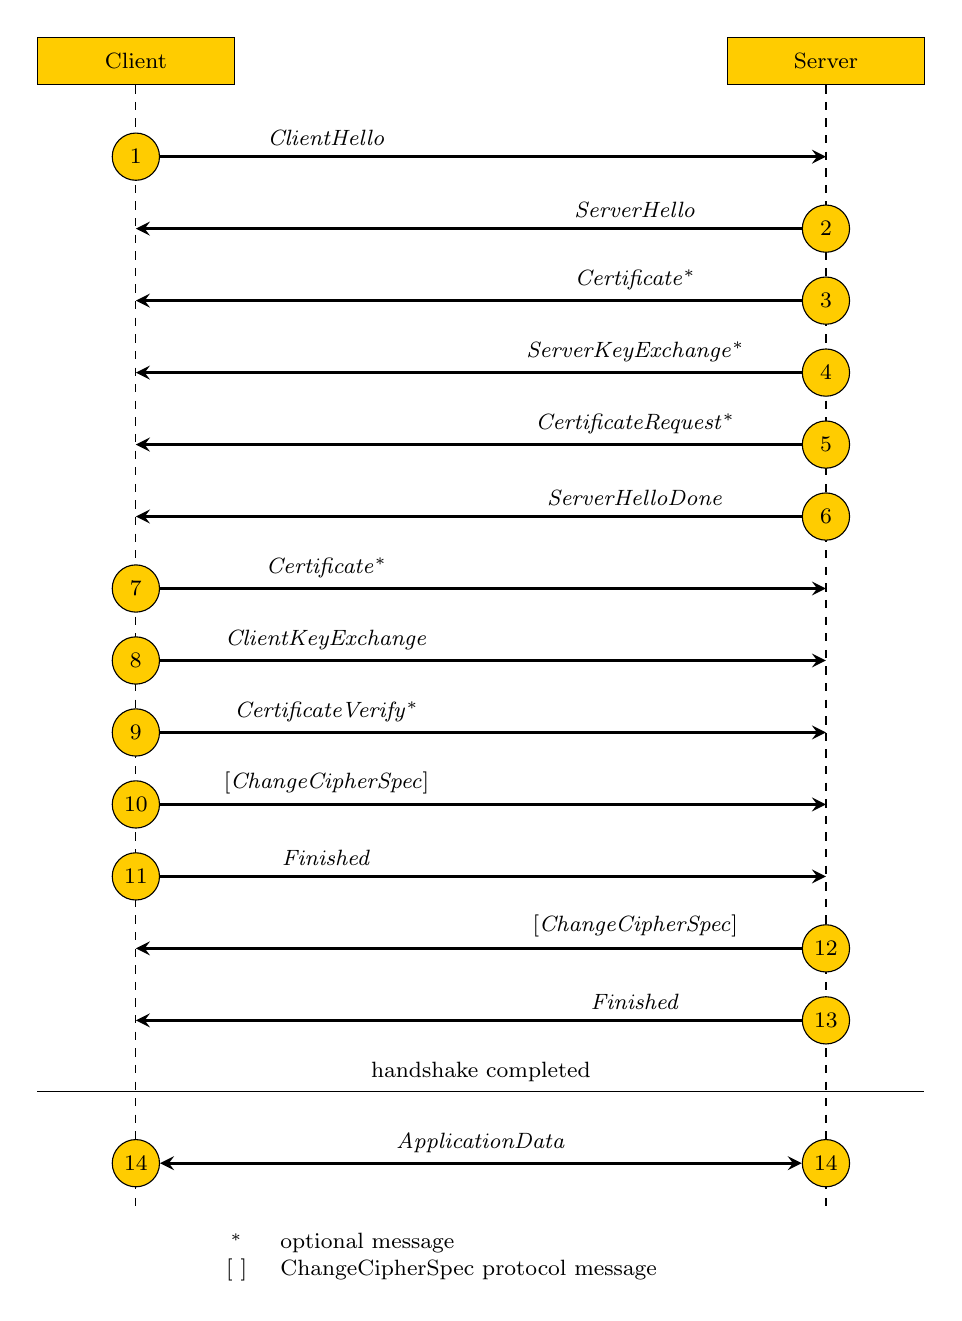
\begin{tikzpicture}
    \node (table) [matrix,row sep=0.5*\nodeheight,column sep=2.5*\nodewidth] {
      \node (client) [rect] {Client}; & \node (server) [rect] {Server}; \\[0.5*\nodeheight]
      \node (client1) [circle] {1}; & \coordinate (server1); \\
      \coordinate (client2); & \node (server2) [circle] {2}; \\
      \coordinate (client3); & \node (server3) [circle] {3}; \\
      \coordinate (client4); & \node (server4) [circle] {4}; \\
      \coordinate (client5); & \node (server5) [circle] {5}; \\
      \coordinate (client6); & \node (server6) [circle] {6}; \\
      \node (client7) [circle] {7}; & \coordinate (server7); \\
      \node (client8) [circle] {8}; & \coordinate (server8); \\
      \node (client9) [circle] {9}; & \coordinate (server9); \\
      \node (client10) [circle] {10}; & \coordinate (server10); \\
      \node (client11) [circle] {11}; & \coordinate (server11); \\
      \coordinate (client12); & \node (server12) [circle] {12}; \\
      \coordinate (client13); & \node (server13) [circle] {13}; \\[0.5*\nodeheight]
      \coordinate (client13b); & \coordinate (server13b); \\[0.5*\nodeheight]
      \node (client14) [circle] {14}; & \node (server14) [circle] {14}; \\
      \coordinate (client15); & \coordinate (server15); \\
    };

    \begin{pgfonlayer}{bg}
      \path [draw,dashed] (client) -- (client15);
      \path [draw,dashed] (server) -- (server15);
    \end{pgfonlayer}
    \path [line] (client1) -- (server1) node[above,near start] {\textit{ClientHello}};
    \path [line] (server2) -- (client2) node[above,near start] {\textit{ServerHello}};
    \path [line] (server3) -- (client3) node[above,near start] {\textit{Certificate}${}^\ast$};
    \path [line] (server4) -- (client4) node[above,near start] {\textit{ServerKeyExchange}${}^\ast$};
    \path [line] (server5) -- (client5) node[above,near start] {\textit{CertificateRequest}${}^\ast$};
    \path [line] (server6) -- (client6) node[above,near start] {\textit{ServerHelloDone}};
    \path [line] (client7) -- (server7) node[above,near start] {\textit{Certificate}${}^\ast$};
    \path [line] (client8) -- (server8) node[above,near start] {\textit{ClientKeyExchange}};
    \path [line] (client9) -- (server9) node[above,near start] {\textit{CertificateVerify}${}^\ast$};
    \path [line] (client10) -- (server10) node[above,near start] {[\textit{ChangeCipherSpec}]};
    \path [line] (client11) -- (server11) node[above,near start] {\textit{Finished}};
    \path [line] (server12) -- (client12) node[above,near start] {[\textit{ChangeCipherSpec}]};
    \path [line] (server13) -- (client13) node[above,near start] {\textit{Finished}};
    \path [draw] ($(client13b)-(0.5*\nodewidth,0)$) -- ($(server13b)+(0.5*\nodewidth,0)$) node[above,midway] {handshake completed};
    \path [line,<->] (client14) -- (server14) node[above,midway] {\textit{ApplicationData}};

    \node [below=0 of table,xshift=-5mm] {
      \begin{tabular}{cl}
        ${}^\ast$ & optional message \\
        $[$ $]$ & ChangeCipherSpec protocol message \\
      \end{tabular}
    };
  \end{tikzpicture}
  \caption{TLS full handshake}
  \label{figures/tls-full-handshake}
\end{figure}

\begin{figure}
  \centering
  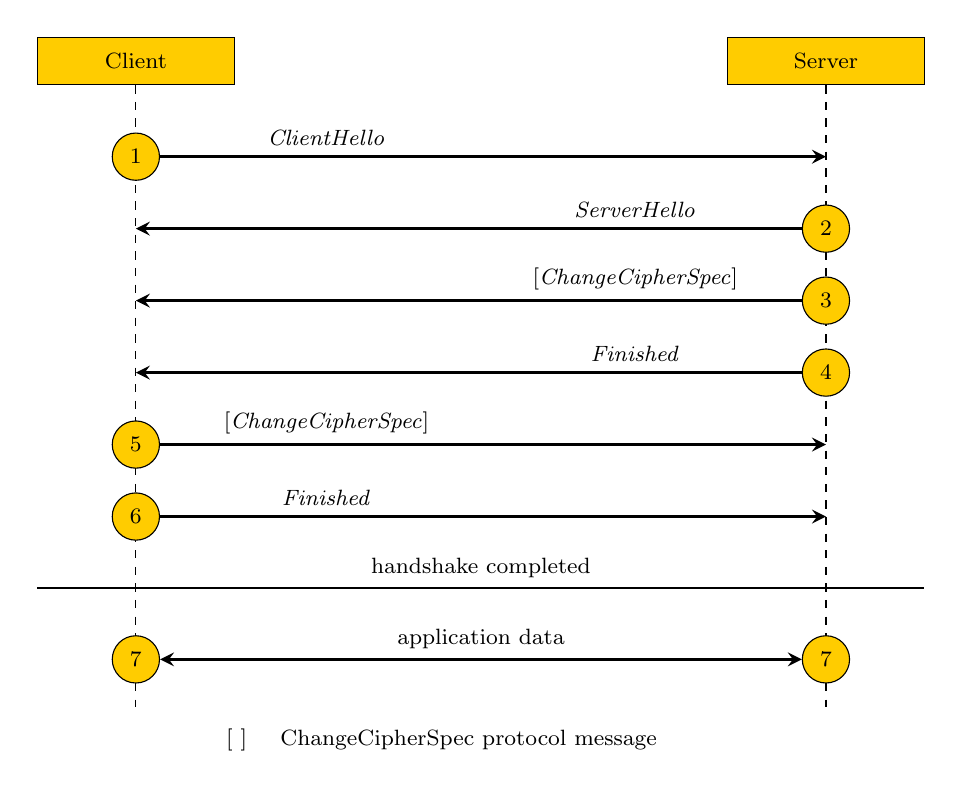
\begin{tikzpicture}
    \node (table) [matrix,row sep=0.5*\nodeheight,column sep=2.5*\nodewidth] {
      \node (client) [rect] {Client}; & \node (server) [rect] {Server}; \\[0.5*\nodeheight]
      \node (client1) [circle] {1}; & \coordinate (server1); \\
      \coordinate (client2); & \node (server2) [circle] {2}; \\
      \coordinate (client3); & \node (server3) [circle] {3}; \\
      \coordinate (client4); & \node (server4) [circle] {4}; \\
      \node (client5) [circle] {5}; & \coordinate (server5); \\
      \node (client6) [circle] {6}; & \coordinate (server6); \\[0.5*\nodeheight]
      \coordinate (client6b); & \coordinate (server6b); \\[0.5*\nodeheight]
      \node (client7) [circle] {7}; & \node (server7) [circle] {7}; \\
      \coordinate (client8); & \coordinate (server8); \\
    };

    \begin{pgfonlayer}{bg}
      \path [draw,dashed] (client) -- (client8);
      \path [draw,dashed] (server) -- (server8);
    \end{pgfonlayer}
    \path [line] (client1) -- (server1) node[above,near start] {\textit{ClientHello}};
    \path [line] (server2) -- (client2) node[above,near start] {\textit{ServerHello}};
    \path [line] (server3) -- (client3) node[above,near start] {[\textit{ChangeCipherSpec}]};
    \path [line] (server4) -- (client4) node[above,near start] {\textit{Finished}};
    \path [line] (client5) -- (server5) node[above,near start] {[\textit{ChangeCipherSpec}]};
    \path [line] (client6) -- (server6) node[above,near start] {\textit{Finished}};
    \path [draw] ($(client6b)-(0.5*\nodewidth,0)$) -- ($(server6b)+(0.5*\nodewidth,0)$) node[above,midway] {handshake completed};
    \path [line,<->] (client7) -- (server7) node[above,midway] {application data};

    \node [below=0 of table,xshift=-5mm] {
      \begin{tabular}{cl}
        $[$ $]$ & ChangeCipherSpec protocol message \\
      \end{tabular}
    };
  \end{tikzpicture}
  \caption{TLS abbreviated handshake}
  \label{figures/tls-abbreviated-handshake}
\end{figure}


If a client and server hasn't previously communicated with each other, both parties will perform a full or basic handshake in order to establish a session. See \autoref{figures/tls-full-handshake}.

Full handshake requires client authentication, whereas basic handshake does not. Also it is possible to perform an anonymous handshake without any authentication, but it is not recommended, because it is sucpectible to MitM attacks.

A full handshake is completed after 4 network flights before the handshake is complete and protocol parties can begin to send application data. Thus, using TLS adds a latency penalty of 2 RTTs if the client sends application data first, such as in HTTP protocol.

\begin{enumerate}
  \item \textit{ClientHello} - client initiates a handshake, sends its capabilities to server
  \item \textit{ServerHello} - server selects the best connection parameters supported by both parties
  \item \textit{Certificate} - server sends its certificate chain (only if server authentication is required)
  \item \textit{ServerKeyExchange} - server sends additional information required to generate the master secret (only if it is required by selected cipher suite)
  \item \textit{CertificateRequest} - server requests client authentication and sends requirements for acceptable certificates (only if client authentication is required)
  \item \textit{ServerHelloDone} - server indicates completion of its side of negotiation
  \item \textit{Certificate} - client sends its certificate chain (only if client authentication is required)
  \item \textit{ClientKeyExchange} - client sends additional information required to generate the master secret
  \item \textit{CertificateVerify} - client proves the posession of private key corresponding to the previously sent client certificate (only if client authentication is required)
  \item \textit{ChangeCipherSpec} - client notifies server, that all following messages are encrypted
  \item \textit{Finished} - client sends a MAC of the handshake messages it sent and received
  \item \textit{ChangeCipherSpec} - server notifies client, that all following messages are encrypted
  \item \textit{Finished} - server sends a MAC of the handshake messages it sent and received
  \item handshake is completed, secure communication channel is established, both parties can securely send application data
\end{enumerate}

An abbreviated handshake is completed after 3 network flights, thus adding a latency penalty of just 1 RRT if the client sends application data first. See \autoref{figures/tls-abbreviated-handshake}. The session reuses previously exchanged secret values between the client and server, identified by either \textit{Session Tickets} or \textit{Session Cookies}.


\subsection{ChangeCipherSpec protocol}
\subsection{Alert protocol}
\subsection{Data protocol}

\section{Cryptographic libraries}

\todo{Seznam kryptogracických knihoven, co dělají, jak se liší, kde a jak moc jsou používané}



\subsection{OpenSSL}

OpenSSL project is an open-source implementation of a lot of cryptographic algorithms and the SSL/TLS protocol. Today, OpenSSL is the most commonly deployed library for SSL/TLS world-wide, both on the server side and in many client tools. Also the commandline tools provided by OpenSSL are also the most common choice for key and certificate management as well as for testing.

Getting started with OpenSSL is very easy, because OpenSSL is preinstalled on the most of Unix operating systems. There are available precompiled binaries for alll common platforms, including Windows.

\subsection{NSS}

\todo{Trochu hlubší popis NSS}

\subsection{Selection}

\todo{which and why I chose}



\chapter{OpenSSL}

OpenSSL\footnote{\url{https://www.openssl.org}} is an opensource cryptographic toolkit, consisting of implementations of many cryptographic aslgorithms, all versions of TLS protocol and various command-line tools.

It is free to get and use for both non-commercial and commercial purposes, with some simple licence conditions\footnote{\url{https://www.openssl.org/source/license.html}}.


\section{Download, build, test, install}

Download the source code from the official OpenSSL homepage\footnote{\url{https://www.openssl.org/source/}} and compare its hash fingerprints. The latest version in the time of writing is 1.0.2a.

Compile it with commands:

\begin{minted}{text}
./config
make
\end{minted}

It results into an all-in-one \texttt{apps/openssl} binary. You can run attached tests with \texttt{make test} command. If you wish to install it globally to your system, run \texttt{make install} command with root privileges.

While making changes into OpenSSL code, sometimes I needed to debug the binary with GDB. You can turn on debugging symbols with \texttt{./config -d} command and build again.


\section{Source code}

OpenSSL source code contains a lot of various directories, for my purposes only the following are significant:

\begin{itemize}
  \item \texttt{apps} -- command-line tools
  \item \texttt{crypto} -- libcrypto library
  \item \texttt{ssl} -- libssl library
  \item \texttt{demos} -- examples
  \item \texttt{docs} -- man pages and howtos
  \item \texttt{include} -- include header files
  \item \texttt{util} -- perl scripts for C code generation
\end{itemize}

OpenSSL provides two primary libraries: libssl and libcrypto. The libcrypto library provides the fundamental cryptographic routines used by libssl. A user can however use libcrypto without using libssl.


\section{Command-line tools}

OpenSSL is primarily a library that is used by developers to include support for strong cryptography in their programs. However it is also a tool that provides access to much of its functionality from command line. This way it can be used by shell scripts or programming languages that do not have native bindings, but can run shell commands. \cite{viega2002network}

The \texttt{openssl} binary is an entry point for all commands. You call it following the pattern:

\begin{minted}{text}
openssl command [command_opts] [command_args]
\end{minted}

Alternatively you can call it without arguments to enter the interactive mode with an \texttt{OpenSSL>} prompt. Then you can directly type your commands. You can leave the interactive mode with Ctrl+C or Ctrl+D or by typing \texttt{quit}.

You can get a list of available commands by calling:

\begin{minted}{text}
openssl list-standard-commands
\end{minted}

OpenSSL binary provides command-line access to the following significant cryptographic operations and applications:

\begin{itemize}
  \item \texttt{openssl dgst} -- a message digest command, producing or verifying a digest of supplied file(s) using hash functions or digital signature algorithms
  \item \texttt{openssl enc} -- a symmetric cipher command, allowing data to be encrypted or decrypted using various block and stream ciphers, using keys derivated from passwords or explicitly provided
  \item \texttt{openssl speed} -- a benchmark to test the performance of all included cryptographic algorithms
  \item \texttt{openssl asn1parse} -- a diagnostic parser of ASN.1 encoded structures; public and private keys, certificates and other cryptographic structures are usually stored in ASN.1 format
  \item \texttt{openssl x509} -- a multi-purpose utility to operate with X509 certificates
  \item \texttt{openssl s\_server} -- a generic TCP+TLS server which listens on a given local port, it can operate either in plain text mode, or as a simple HTTP server, processing requests and responding with files in current directory
  \item \texttt{openssl s\_client} -- a generic TCP+TLS client which connects to a remote host, very useful diagnostic tool
  \item \texttt{openssl s\_time} -- a client which benchmarks the performance of a TLS connection
\end{itemize}

OpenSSL supports a lot of cryptographic algorithms, some of them also have their own aliases (pseudo-commands) for faster command line access. Supported algorithms and their corresponding pseudo-commands can be listed by the following commands:

\begin{itemize}
  \item \texttt{openssl list-message-digest-algorithms} -- list of message digest algorithms
  \item \texttt{openssl list-message-digest-commands} -- list of message digest pseudo-commands
  \item \texttt{openssl list-cipher-algorithms} -- list of symmetric encryption algorithms
  \item \texttt{openssl list-cipher-commands} -- list of symmetric encryption pseudo-commands
  \item \texttt{openssl list-public-key-algorithms} -- list of public key algorithms
  \item \texttt{openssl ciphers -v [\textit{cipherlist}]} -- list of TLS cipher suites, complying with the given cipherlist, or all by default
  \item \texttt{openssl ecparam -list\_curves} -- list of named elliptic curves
\end{itemize}


\subsection{Symmetric encryption}
\label{toc/openssl-enc}

The \texttt{openssl enc} command\footnote{\url{https://www.openssl.org/docs/apps/enc.html}} encrypts or decrypts given data using various supported ciphers. By default, it reads the data from standard input, a writes to standard output.

It accepts the following significant options:

\begin{itemize}
  \item \texttt{-\textit{ciphername}} -- the cipher name, it specifies the requirements on the length of key and IV
  \item \texttt{-d} -- decrypt the input data
  \item \texttt{-K \textit{hex}} -- the key used in cipher, it must be represented as a string comprised only of hex digits
  \item \texttt{-iv \textit{hex}} -- the IV used in cipher, it must be represented as a string comprised only of hex digits
\end{itemize}

Example:

\inputminted{text}{code/openssl-enc-example.txt}


\subsection{Performance benchmarking of cryptographic algorithms}

The \texttt{openssl speed} command\footnote{\url{https://www.openssl.org/docs/apps/speed.html}} can run performance benchmarks of all included cryptographic algorithms - hash functions, symmetric ciphers, assymetric key exchanges and digital signatures.

It accepts the following significant options:

\begin{itemize}
  \item \texttt{-evp \textit{algorithmname}} -- run benchmarks on an EVP algorithm
  \item \texttt{\textit{algorithmnames}} -- if any algorithms are given, speed tests those algorithms, otherwise all are tested
\end{itemize}

Example:

\inputminted{text}{code/openssl-speed-example.txt}


\subsection{Generic server}
\label{toc/openssl-s_server}

The \texttt{openssl s\_server} command\footnote{\url{https://www.openssl.org/docs/apps/s\_server.html}} emulates a generic TCP server, which uses TLS to ensure a secure communication channel. It listens for incoming connections and after a connection is established, it forwards standard input to the opposite party through TLS data protocol, and writes all received data to standard output.

It accepts the following significant options:

\begin{itemize}
  \item \texttt{-accept \textit{port}} -- the port to listen on for connections, 4433 by default
  \item \texttt{-cert \textit{filename}} -- the certificate, a self-signed certificate can be used
  \item \texttt{-key \textit{filename}} -- the certificate private key
  \item \texttt{-cipher \textit{ciphernames}} -- the supported cipher list. When the client sends a list of supported ciphers, the first client cipher also included in the server list is chosen. Because the client specifies the preference order, the order of the server cipherlist irrelevant. This behavior can be overriden by \texttt{-serverpref} option.
  \item \texttt{-serverpref} -- use the server's cipher preferences, rather than the client's preferences
  \item \texttt{-WWW} -- emulates a simple web server. Resources will be resolved relative to the current directory, for example if the resource \texttt{/page.html} is requested, the file \texttt{./page.html} will be loaded.
\end{itemize}

Example, run in parallel with \texttt{s\_client} example:

\inputminted{text}{code/openssl-s_server-example.txt}

After the connection is established, a string "Lorem ipsum..." is successfully transferred from the client to the server.


\subsection{Generic client}
\label{toc/openssl-s_client}

The \texttt{openssl s\_client} command\footnote{\url{https://www.openssl.org/docs/apps/s\_client.html}} emulates a generic TCP client, which uses TLS to ensure a secure communication channel. After a connection is established, it forwards standard input to the opposite party through TLS data protocol, and writes all received data to standard output.

It accepts the following significant options:

\begin{itemize}
\item \texttt{-connect \textit{host:port}} -- the host and port to connect to, local host and port 4433 by default
\item \texttt{-cipher \textit{ciphernames}} -- the supported cipher list. Although the server determines which cipher suite is used, it should take the first supported cipher in the list sent by the client.
\end{itemize}

Example, run in parallel with \texttt{s\_server} example:

\inputminted{text}{code/openssl-s_client-example.txt}

After the connection is established, a string "Lorem ipsum..." is successfully transferred from the client to the server.


\subsection{Performance benchmarking of TLS}

The \texttt{openssl s\_time} command\footnote{\url{https://www.openssl.org/docs/apps/s\_time.html}} emulates a generic TCP client, which uses TLS to ensure a secure communication channel. It can request a page from the server and includes the time to transfer the payload data in its timing measurements. It measures the number of connections within a given timeframe, the amount of data transferred (if any), and calculates the average time spent for one connection.

It accepts the following significant options:

\begin{itemize}
  \item \texttt{-connect \textit{host:port}} -- the host and port to connect to, local host and port 4433 by default
  \item \texttt{-cipher \textit{ciphernames}} -- the supported cipher list. Although the server determines which cipher suite is used, it should take the first supported cipher in the list sent by the client.
  \item \texttt{-time \textit{sec}} -- specifies how long in seconds the benchmark should run
  \item \texttt{-new} -- performs the timing test using a new session for each connection. If \texttt{-www} option is not used, this can be used to benchmark specifically the TLS handshake protocol.
  \item \texttt{-reuse} -- performs the timing test using the same session for each connection. If \texttt{-www} option is not used, this can be used to benchmark specifically the TLS handshake protocol with session resume.
  \item \texttt{-www \textit{filename}} -- this specifies the resource to GET from the server. If this parameter is not specified, then it will only perform the TLS handshake to establish a connections, but not transfer any data.
\end{itemize}

\inputminted{text}{code/openssl-s_time-example.txt}


\section{libcrypto library}
\label{toc/openssl-libcrypto}

The libcrypto\footnote{\url{https://wiki.openssl.org/index.php/Libcrypto_API}} library provides high-level and low-level interfaces for the implemented fundamental cryptographic algorithms.

For most uses, users should use the high-level interface that is provided for performing cryptographic operations. This is known as the EVP\footnote{\url{https://wiki.openssl.org/index.php/EVP}} interface (short for Envelope). This interface provides a suite of functions for performing encryption/decryption (both symmetric and asymmetric), signing/verifying, as well as generating hashes and MAC codes, across the full range of OpenSSL supported algorithms and modes. Working with the high-level interface means that a lot of the complexity of performing cryptographic operations is hidden from view. A single consistent API is provided. In the event that you need to change your code to use a different algorithm (for example), then this is a simple change when using the high-level interface. In addition low-level issues such as padding and encryption modes are all handled for you.

The EVP functions provide a high-level interface to OpenSSL cryptographic functions. They provide the following features:

\begin{itemize}
  \item A single consistent interface regardless of the underlying algorithm or mode
  \item Support for an extensive range of algorithms
  \item Encryption/Decryption using both symmetric and asymmetric algorithms
  \item Sign/Verify
  \item Key derivation
  \item Secure Hash functions
  \item Message Authentication Codes
  \item Support for external crypto engines
\end{itemize}

In addition to the high-level interface, OpenSSL also provides low-level interfaces for working directly with the individual algorithms. These low-level interfaces are not recommended for the novice user, but provide a degree of control that may not be possible when using only the high-level interface.

Where possible, the high-level EVP interface should be used in preference to the low-level interfaces. This is because the code then becomes transparent to the algorithm used and much more flexible. Additionally, the EVP interface will ensure the use of platform specific cryptographic acceleration such as AES-NI. The low-level interfaces do not provide the guarantee.


\subsection{EVP API}
\label{toc/openssl-evp}

A specific cipher or message digest algorithm is identified by an unique \texttt{EVP\_CIPHER} or \texttt{EVP\_MD} struct respectively. OpenSSL user is not expected to create these themself, but instead they can use a built-in function to return the struct of particular algorithm that they wish to use. In the following text I focus only on cipher algorithms.

An extract from \texttt{evp.h} header file listing some functions returning \texttt{EVP\_CIPHER} struct is shown below. There is a specific function for every supported combination of cipher algorithm and its parameters (a key length, a block mode, etc.).

\inputminted{c}{code/openssl-evp-ciphers.c}

The \texttt{EVP\_CIPHER} is represented by the following signature:

\inputminted{c}{code/openssl-evp-cipher.c}

The meaning of its important parameters follows:

\begin{itemize}
  \item \texttt{nid} -- integer; unique identifier
  \item \texttt{block\_size} -- integer; cipher block size
  \item \texttt{key\_len} -- integer; cipher key length
  \item \texttt{iv\_len} -- integer; cipher IV length
  \item \texttt{flags} -- bit array, represented as integer; cipher flags specifying its capabilities
  \item \texttt{init} -- function pointer; called during initialization, it can allocate the cipher context before the operation
  \item \texttt{do\_cipher} -- function pointer; called during sending the input data, it should perform the encrypt/decrypt operation
  \item \texttt{cleanup} -- function pointer; called during finalization, it can free the cipher context after the operation
  \item \texttt{ctx\_size} -- integer; cipher-specific context size, can be used to store cipher-specific data during the operation
  \item \texttt{ctrl} -- function pointer; used to invoke special actions, which don't have a specific field in the \texttt{EVP\_CAESAR} struct
\end{itemize}

Prior to performing the encrypt/decrypt operation, a cipher context must be allocated and initialized to store setting and state during the operation. The cipher context is represented by \texttt{EVP\_CIPHER\_CTX} struct.

\inputminted{c}{code/openssl-evp-cipher-ctx-new.c}

Note the cipher context is different from cipher-specific context. The cipher-specific context is stored inside of the cipher context, however the cipher-specific context is allocated and freed by the cipher itself in its \texttt{init} and \texttt{cleanup} functions, which are called by EVP internally, and a user doesn't need to care about it.

So now we are prepared to perform the encrypt/decrypt operation. First, we need to set a cipher, a secret key and an initialization vector (IV). We can use an initialization function, specifically named \texttt{EVP\_EncryptInit\_ex} or \texttt{EVP\_DecryptInit\_ex}. There is also an universal \texttt{EVP\_CipherInit\_ex} function with \texttt{enc} parameter, which controls which operation is performed. However I recommend the first option, because usually we are sure which operation do we want to perform, so it should be hardcoded using the specific functions instead of depending of an integer parameter. It internally calls the cipher's \texttt{init} function from the \texttt{EVP\_CIPHER} struct.

\inputminted{c}{code/openssl-evp-cipherinit.c}

Any input data should be sent to the cipher by an update function \texttt{EVP\_EncryptUpdate} or \texttt{EVP\_DecryptUpdate}. It accepts the input data, and it fills the provided output buffer with the encrypted/decrypted output data, and returns a number of written bytes. Usualy it can be called multiple times, if the cipher supports streaming.

The functions internally calls the cipher's \texttt{do\_cipher} function with the same parameters.

\inputminted{c}{code/openssl-evp-cipherupdate.c}

After the input data block ends, a finalization function \texttt{EVP\_EncryptFinal\_ex} or \texttt{EVP\_DecryptFinal\_ex} needs to be called. This function can append few more bytes to output, for example a padding or an authentication tag.

The functions internally call the cipher's \texttt{do\_cipher} function with null parameters to signalize the end of operation. The cipher can react by appending few more bytes to output, for example a padding or an authentication tag.

\inputminted{c}{code/openssl-evp-cipherfinal.c}

After all cipher operations were finished, the cipher context must be cleaned up and freed by the \texttt{EVP\_CIPHER\_CTX\_free} function. It internally calls the cipher's \texttt{cleanup} function.

\inputminted{c}{code/openssl-evp-cipher-ctx-free.c}


\subsection{EVP API -- Symmetric encryption and decryption}
\label{toc/openssl-evp-encryption}

With the knowledge of EVP API as described in \autoref{toc/openssl-evp}, a user can perform symmetric encryption and decryption operations across a wide range of algorithms and modes. The following code shows how to use it to encrypt and decrypt a piece of confidential information.

Encryption using the EVP API consists of the following stages:

\begin{itemize}
  \item Setting up a cipher context
  \item Initializing the encryption operation, providing key, IV
  \item Providing plaintext bytes to be encrypted
  \item Finalizing the encryption operation
\end{itemize}

The sample \texttt{encrypt} function uses AES-128 in CBC mode. It takes as arguments the plaintext, the length of the plaintext, the key, and the IV. Also it takes in a buffer to put the ciphertext in (which we assume to be long enough), and will return the length of the ciphertext that it writtes.

The length of plaintext is necessary, OpenSSL can't use \texttt{strlen} function to determine its length, because it can contain any data, even null (\texttt{\textbackslash0}) bytes. The length of key and IV is fixed, appropriate for the chosen cipher, which means both the key and IV 16 bytes long for AES-128 in CBC mode.

The source code follows. It misses the most of error handling code, which would be necessary in a real application.

\inputminted{c}{code/openssl-evp-encrypt.c}

Decryption using the EVP API consists of the following steps:

\begin{itemize}
  \item Setting up a cipher context
  \item Initializing the decryption operation, providing key, IV
  \item Providing ciphertext bytes to be decrypted
  \item Finalizing the decryption operation
\end{itemize}

The sample \texttt{decrypt} function uses AES-128 in CBC mode. It takes almost the same arguments as the \texttt{encrypt} function, with the exception that the plaintext and the ciphertext are swapped.

The source code follows. It misses the most of error handling code, which would be necessary in a real application.

\inputminted{c}{code/openssl-evp-decrypt.c}


\subsection{EVP API -- Authenticated encryption and decryption}
\label{toc/openssl-evp-aead-encryption}

Following the recent advances in AEAD, the EVP API of libcrypto library also supports the ability to perform authenticated encryption and decryption. It provides confidentiality by encrypting the data, and authenticity by creating a MAC tag over the encrypted data.

Using AEAD ciphers is nearly identical to using standard symmetric encryption ciphers. In addition, a user can optionally provide some Additional Authenticated Data (AAD). The AAD data is not encrypted, and is typically passed to the recipient in plaintext along with the ciphertext. An example of AAD is the IP address and port number in a IP header used with IPsec.

The output from the encryption operation will be the ciphertext, and a MAC tag. The MAC tag is subsequently used during the decryption operation to ensure that the ciphertext and AAD have not been tampered with.

Authenticated encryption using the EVP API in much the same way as for symmetric encryption as described in \autoref{toc/openssl-evp-encryption}. The main differences are:

\begin{itemize}
  \item AAD data can be provided before encrypting the plaintext data
  \item after the encryption is finished, the MAC tag needs to be obtained
\end{itemize}

The sample \texttt{encrypt} function uses AES-128 in GCM mode. It takes as arguments the plaintext, the length of the plaintext, the key, and the IV. Also it takes in a buffer to put the ciphertext and the MAC tag in (which we assume to be long enough), and will return the length of the ciphertext that it writtes.

The length of plaintext is necessary, OpenSSL can't use \texttt{strlen} function to determine its length, because it can contain any data, even null (\texttt{\textbackslash0}) bytes. The length of key, IV and MAC tag is fixed, appropriate for the chosen cipher, which means the key 16 bytes long, the IV 12 bytes long and the MAC tag 16 bytes for AES-128 in GCM mode by default.

The source code follows. It misses the most of error handling code, which would be necessary in a real application.

\inputminted{c}{code/openssl-evp-aead-encrypt.c}

Authenticated decryption using the EVP API in much the same way as for symmetric decryption as described in \autoref{toc/openssl-evp-encryption}. The main differences are:

\begin{itemize}
  \item AAD data can be provided before decrypting the ciphertext data
  \item before the decryption is finished, the expected MAC tag needs to be provided
  \item a return value should be considered as a possible failure to authenticate ciphertext and/or AAD
\end{itemize}

The sample \texttt{decrypt} function uses AES-128 in GCM mode. It takes almost the same arguments as the \texttt{encrypt} function, with the exception that the plaintext and the ciphertext are swapped, and the MAC tag is provided by a user.

The source code follows. It misses the most of error handling code, which would be necessary in a real application.

\inputminted{c}{code/openssl-evp-aead-decrypt.c}

Currently, there is no standardized way to get and set the MAC tag for different ciphers. All current implementations use the universal \texttt{EVP\_CIPHER\_CTX\_ctrl} function, which allows various cipher specific actions. However, the action identifier is specific for each cipher, e.g. \texttt{EVP\_CTRL\_GCM\_GET\_TAG}. This should change in future version of OpenSSL, there are new universal action identifiers such as \texttt{EVP\_CTRL\_AEAD\_GET\_TAG} in development code, used by both currently implemented AEAD ciphers (AES-GCM, AES-CCM).


\section{libssl library}

\chapter{Implementing a new TLS cipher suite in OpenSSL}

All CAESAR candidates publish its encrypt/decrypt primitives through the same CAESAR API, see \autoref{toc/caesar-api}. I decided to implement a generic TLS cipher suite into OpenSSL in such way, that any CAESAR candidate can be used in the new cipher suite.

This chapter documents my source code added to OpenSSL 1.0.2. Basically I implemented a bridge between OpenSSL EVP API and CAESAR API. I can compile my customized OpenSSL with any CAESAR cipher, and it works. For my testing purposes, I chose the NORX cipher, see \autoref{toc/caesar-selection}.

There is no public documentation about implementing a new cipher or a new TLS cipher suite into OpenSSL, so I had to read through the OpenSSL source code a lot, tracing the code of already implemented ciphers and cipher suites.

The OpenSSL code is a joint work of many security experts, verified by real-world production usage and it can contain a lot of undocumented hidden knowledge. Because of no public documentation about this topic, I consider my implementation as experimental and O'm sure that my implementation is not perfect, it can contain hidden security bugs. Having this in mind, \textbf{I don't recomment my code for production under any circumstances.}

\section{Cipher}
\label{toc/implementation-cipher}

EVP API provides an universal interface to symmetric encryption, here a source code using it is independent on the chosen cipher. This is the main reason why I chose to implement a new cipher into the OpenSSL EVP API.

EVP API is a high-level interface to OpenSSL cryptographic functions. While OpenSSL also has direct interfaces for cryptographic operations, the EVP interface separates the operations from the actual backend used. That way, the actual implementation that is used can be changed, and one can specify an engine to use for the operations.

\subsection{Implementation}

I implemented a new abstract cipher named CAESAR, which serves as a bridge to its real implementation behind CAESAR API. Source code shown here is stripped to the most important parts, for full source code see attached files of this thesis.

I defined a new function in \texttt{crypto/evp/evp.h} file returning a reference to my new \texttt{EVP\_CIPHER} struct.

\inputminted{c}{code/openssl-evp-caesar.c}

I implemented all cipher related code in \texttt{crypto/evp/caesar/e\_caesar.c} file. The cipher is defined by an \texttt{EVP\_CIPHER} struct, which holds all cipher-cpecific setting and pointers to functions performing related operations. See \autoref{toc/openssl-libcrypto} for more detailed description of the EVP API.

\inputminted{c}{code/openssl/crypto/evp/caesar/e_caesar.c}

The cipher's \texttt{init} function (specifically \texttt{caesar\_init}) initializes the cipher context in \texttt{EVP\_CAESAR\_CTX} struct, and copies the key and the IV into the context, so it can be used later by the \texttt{caesar\_cipher} function.

\inputminted{c}{code/openssl/crypto/evp/caesar/e_caesar_init.c}

The cipher's \texttt{do\_cipher} function (specifically \texttt{caesar\_cipher}) is the main processing function. It applies the cipher to the input data, and writes the result of the encrypt/decrypt operation to the output buffer. If the function is called with no output buffer, the input data is considered as associated data, which contributes to MAC tag.

\inputminted{c}{code/openssl/crypto/evp/caesar/e_caesar_cipher.c}
\inputminted{c}{code/openssl/crypto/evp/caesar/e_caesar_set_ad.c}
\inputminted{c}{code/openssl/crypto/evp/caesar/e_caesar_encrypt.c}
\inputminted{c}{code/openssl/crypto/evp/caesar/e_caesar_decrypt.c}

The cipher's \texttt{cleanup} function (specifically \texttt{caesar\_cleanup}) is used to cleanup and free all memory allocated by init functions.

\inputminted{c}{code/openssl/crypto/evp/caesar/e_caesar_cleanup.c}

The cipher's \texttt{ctrl} function (specifically \texttt{caesar\_ctrl}) is used to invoke special actions, which don't have a specific field in the \texttt{EVP\_CIPHER} struct. I needed only one specific action, \texttt{EVP\_CTRL\_AEAD\_TLS1\_AAD} for setting associated data from TLS library.

\inputminted{c}{code/openssl/crypto/evp/caesar/e_caesar_ctrl.c}

Finally I registered the new cipher in \texttt{crypto/evp/c\_allc.c} file. From now on, the new cipher is available for use by its name, \texttt{caesar}.

\inputminted{c}{code/openssl/crypto/evp/c_allc.c}

\subsection{Testing}

First I checked if the new cipher is registered properly in OpenSSL.

\inputminted{text}{code/caesar-list-cipher-algorithms.txt}

I created a simple Shell script to test my new cipher. It uses a fixed sample plaintext, and it generates a random key and IV.

It uses OpenSSL CLI command \texttt{enc} as described in \autoref{toc/openssl-enc}. It encrypts and decrypts a sample plaintext with my new \texttt{caesar} cipher.

In order to verify that my new cipher implementation works as intended, the following criterias must pass:

\begin{itemize}
  \item no error is thrown \\ An error can be thrown because of various reasons:
  \begin{itemize}
    \item the new cipher is not implemented correctly
    \item invalid padding found during decryption
    \item invalid MAC tag found during decryption
  \end{itemize}
  \item the output plaintext from decrypt operation equals to the original plaintext
  \item if any of the key, the IV, and the input plaintext changes, the ciphertext output changes as well
  \item if the key and IV is set to a fixed value, the ciphertext output from encrypt operation should stay the same
\end{itemize}

\inputminted{bash}{code/test-enc.sh}

The script's output follows.

\inputminted{text}{code/test-enc.sh.out}

Note that OpenSSL CLI \texttt{enc} command currently doesn't support any way to provide additional authenticated data. Actually it doesn't support AEAD ciphers at all, there is a condition checking for AEAD flag in the cipher's flags field, which throws an error. I commented off this condition, because I needed this command to test the new cipher. There is no harm in doing so, additional authenticated data can be empty, and the MAC tag is still checked by the cipher itself.

\inputminted{c}{code/openssl/apps/enc.c}


\section{TLS cipher suite}
\label{toc/implementation-cipher-suite}

Any TLS cipher suite consists of various selected cryptographic primitives, providing key exchange, authentication, encryption and MAC. My thesis focuses only on a new encryption algorithm, so I implemented a new TLS cipher suite, which consists of a secure choice of Diffie-Hellman ephemeral (DHE) key exchange, RSA authentication, CAESAR encryption (see \autoref{toc/implementation-cipher} for details about implementation) and SHA256 pseudorandom function. There is no MAC, because MAC is already provided by the CAESAR AEAD cipher itself.

I named the new cipher suite to be consistent with existing cipher suites, \texttt{TLS\_DHE\_RSA\_WITH\_CAESAR\_SHA256} by IANA conventions and \texttt{DHE-RSA-CAESAR-SHA256} by OpenSSL conventions.

The new cipher suite which can be negotiated by client and server in TLS handshake (see \autoref{toc/tls-handshake} for details). During the handshake, cipher suites are represented by IDs. Public cipher suites are registered by IANA organization\footnote{\url{http://www.iana.org/assignments/tls-parameters/tls-parameters.xhtml}} and they are assigned with unique IDs, which are known to all parties. I didn't want to publish the new cipher suite to production, I consider it experimental, so I used a private space of IDs: \textit{"All cipher suites whose first byte is 0xFF are considered private and can be used for defining local/experimental algorithms."} \cite{rfc2246} So I chose the ID for the new cipher suite to be \texttt{FF81}.

\subsection{Implementation}

OpenSSL code related to TLS cipher suites is capable of using EVP API, thus it was really simple to implement the new cipher suite using the new cipher from \autoref{toc/implementation-cipher}.

First I added a few new constants to \texttt{ssl/tls1.h}, \texttt{ssl/ssl\_locl.h} and \texttt{ssl/t1\_trce.c} files, defining IDs and names of the new cipher suite.

\inputminted{c}{code/openssl/ssl/tls1.h}
\inputminted{c}{code/openssl/ssl/ssl_locl.h}
\inputminted{c}{code/openssl/ssl/t1_trce.c}

I added a new cipher suite definition to \texttt{ssl/s3\_lib.c} file, where I referenced the new cipher using the new constants.

\inputminted{c}{code/openssl/ssl/s3_lib.c}

In \texttt{ssl/ssl\_ciph.c} file I found every code responsible for finding a correct EVP cipher by the new constants, and I added there a condition branch returning the new cipher.

\inputminted{c}{code/openssl/ssl/ssl_ciph.c}

\subsection{Testing}

I used OpenSSL CLI commands \texttt{s\_server} and \texttt{s\_client} as described in \autoref{toc/openssl-s_server} and \autoref{toc/openssl-s_client}. I run them simultaneously, each command in a separate terminal on a single computer. Server and client are connected to each other byu specifying the same single port \texttt{4444}.

The \texttt{s\_server} command creates a TCP server. It listens on a specified port (\texttt{4444}) and forces negotiation of the new ciphersuite \texttt{DHE-RSA-CAESAR-SHA256}. It authenticates itself by a self-signed certificate, which I created only for purpose of testing the new cipher suite.

The \texttt{s\_client} command creates a TCP client. It connects to the specified host and port (\texttt{localhost:4444}) and forces negotiation of the new ciphersuite \texttt{DHE-RSA-CAESAR-SHA256}.

In order to verify that my new cipher implementation works as intended, the following criterias must pass:

\begin{itemize}
  \item no error is thrown \\ An error can be thrown because of various reasons:
  \begin{itemize}
    \item the new cipher is not implemented correctly (this was verified in \autoref{toc/implementation-cipher})
    \item the new cipher suite is not implemented correctly
  \end{itemize}
  \item a two-way \textbf{communication channel} between the server and client is established \\ Any data that I enter on server will be sent \textbf{unaltered} to client and vice versa.
  \item a two-way \textbf{secure communication channel} between the server and client is established \\ Any data that I send via the channel will be sent \textbf{encrypted} during transmission.
\end{itemize}

I entered a fixed message (\textit{"Lorem ipsum dolor sit amet, consectetur adipiscing elit.\textbackslash{}n"}) to client and I watched it appear on server. The output from server and client reports that it is using the new cipher suite. The communication channel was successfully established.

\inputminted{text}{code/caesar-s_client.txt}
\inputminted{text}{code/caesar-s_server.txt}

I watched the communication using the Wireshark application, which is capable of monitoring network traffic. It shows the TLS Handshake protocol (as described in \autoref{toc/tls-handshake}) messages negotiating the new cipher suite identified by ID \texttt{FF81} and the TLS Application protocol messages carrying the encrypted data.

In Wireshark, I logged all communication on local loopback network interface and filtered all TLS communication. See the packet capture \autoref{table/packet-capture}. For the purpose of verifying my implementation, there are following important packets with TLS protocol messages:

\begin{table}
  \centering

  \begin{tabularx}{\textwidth}{rllX}
    \csvtable{tables/packets.csv}
      {No. & Source & Destination & Content}
      {\csvcoli & \csvcolii & \csvcoliii & \csvcoliv}
  \end{tabularx}

  \caption{Packet capture}
  \label{table/packet-capture}
\end{table}


\begin{itemize}
  \item Packet 4 -- ClientHello
  \item Packet 6 -- ServerHello
  \item Packet 7 -- ChangeCipherSpec
  \item Packet 8 -- ChangeCipherSpec
  \item Packet 11 -- ApplicationData
\end{itemize}

When the client initiates the connection, it sends the ClientHello message. It contains client's capabilites. The most important for me is the list of supported cipher suites. There is an unknown cipher suite \textit{"Unknown (0xff81)"}, which represents the new cipher suite.

\inputminted{text}{code/packet-client-hello.txt}

The server receives the ClientHello message, compares the client's capabilities with its own, selects the best connection parameters which are supported by both parties, and sends them back to the client in the ServerHello message. Again, there is an unknown cipher suite \textit{"Unknown (0xff81)"}, which represents the new cipher suite.

\inputminted{text}{code/packet-server-hello.txt}

The client and server now performs a check if the secret communication channel was sucessfully established. They send a ChangeCipherSpec message signalizing that all subsequent communitaion is encrypted by the selected cipher suite and a Finished message containing some data known to both parties. If decryption succeeds, they can start transmitting ApplicationData messages.

There is a single ApplicationData message which doesn't contain any plaintext data. Nobody should be able to decrypt it, because the secret key is exchanged assymetrically by Diffie-Hellman algorithm. I can confirm that it contains my message by comparing plaintext and ciphertext lengths.

\inputminted{text}{code/packet-data.txt}

The plaintext message sent from client to server is 57 bytes long. The ciphertext as observed in packet capture is 73 bytes long. The cipher is an AEAD stream cipher with MAC tag 16 bytes long, thus the ciphertext length should equal the plaintext length + the MAC tag length. $L_{ciphertext} = L_{plaintext} + L_{MAC}$, $73 + 57 + 16$ It confirms that my implementation works as intended.

\begin{conclusion}

The TLS protocol consists of a complex structure of standardized RFC documents by IETF. I studied the most important ones to understand the flow of the TLS protocol over the network. I examined its implementation in the OpenSSL library, which consists of a complicated, decades-old C code. Nonetheless this library is massively used in the real world and it is an important part of critical infrastructure of the Internet.

I studied the field of authenticated encryption while following the course of the CAESAR competition and recently published relevant papers. I classified CAESAR submissions by their design principles, overall construction and underlying primitives. I presented functional requirements and selection criteria for the winning candidates.

During the time of writing this thesis, the announcement of second-round candidates keeps being postponed. I did not have enough information to make a quallified choice, so I decided to implement a cipher using the generic CAESAR API.

As a reference for my implementation I chose the NORX cipher, because it has received no negative analysis. However it is not important which particular cipher I used. It can be easily substituted for a different one complying with the CAESAR API, as soon as the second-round or the final candidates are announced.

I successfully tested my implementation by observing TLS network communication between server and client.

\end{conclusion}

%\nocite{*}
\bibliographystyle{alpha}
\bibliography{DP_Zak_Jan_2015}

\appendix
\chapter{Symbols}

\begin{description}
  \item[$m$] plaintext message
  \item[$c$] ciphertext message
  \item[$a$] message authentication code
  \item[$E$] encrypt function
  \item[$D$] decrypt function
  \item[$H$] hash function
  \item[$S$] sign function
  \item[$V$] verify function
  \item[$K$] secret shared key
  \item[$PK$] public key
  \item[$SK$] secret (private) key
\end{description}

\chapter{Acronyms}

\begin{description}
  \item[AAD] Additional Authenticated Data
  \item[AE] Authenticated Encryption
  \item[AEAD] Authenticated Encryption with Associated Data
  \item[AES] Anvanced Encryption Standard
  \item[AES-NI] Advanced Encryption Standard - New Instructions
  \item[AVX] Advanced Vector Extensions
  \item[CAESAR] Competition for Authenticated Encryption: Security, Applicability and Robustness
  \item[DTLS] Datagram Transport Layer Security
  \item[EtM] Encrypt-then-MAC
  \item[HTTP] Hypertext Transfer Protocol
  \item[HTTPS] Hypertext Transfer Protocol Secure
  \item[IETF] Internet Engineering Task Force
  \item[IP] Internet Protocol
  \item[ISO] International Organization for Standardization
  \item[IV] Initialization Vector
  \item[MAC] Message Authentication Code
  \item[MitM] Man-in-the-Middle
  \item[M\&E] MAC-and-Encrypt
  \item[MtE] MAC-then-Encrypt
  \item[OTP] One-Time Pad
  \item[PRF] Pseudorandom Function
  \item[RFC] Request for Comments
  \item[RTT] Round-Trip Time
  \item[SIMD] Single Instruction Multiple Data
  \item[SSE] Streaming SIMD Extensions
  \item[SSH] Secure Shell
  \item[SSL] Secure Sockets Layer
  \item[TCP] Transmission Control Protocol
  \item[TLS] Transport Layer Security
  \item[UDP] User Datagram Protocol
\end{description}

\chapter{TLS constants}

\begin{table}
  \centering

  \begin{tabular}{ccl}
    \csvtable{tables/tls-record-types.csv}
      {Dec & Hex & Name}
      {\csvcoli & \texttt{\csvcolii} & \csvcoliii}
  \end{tabular}

  \caption{TLS record types}
  \label{figure/tls-record-types}
\end{table}

\begin{table}
  \centering

  \begin{tabular}{cccl}
    \csvtable{tables/tls-versions.csv}
      {Major & Minor & Hex & Name}
      {\csvcoli & \csvcolii & \texttt{\csvcoliii} & \csvcoliv}
  \end{tabular}

  \caption{TLS versions}
\end{table}

\begin{table}
  \centering

  \begin{tabular}{ccl}
    \csvtable{tables/tls-handshake-message-types.csv}
      {Dec & Hex & Name}
      {\csvcoli & \texttt{\csvcolii} & \csvcoliii}
  \end{tabular}

  \caption{TLS handshake message types}
\end{table}

\begin{table}
  \centering

  \begin{tabular}{cclp{7.75cm}}
    \csvtable{tables/tls-alert-message-levels.csv}
      {Dec & Hex & Name}
      {\csvcoli & \texttt{\csvcolii} & \csvcoliii}
  \end{tabular}

  \caption{TLS alert message levels}
\end{table}

\begin{table}
  \centering

  \begin{tabular}{ccll}
    \csvtable{tables/tls-alert-message-types.csv}
      {Dec & Hex & Name & Level}
      {\csvcoli & \texttt{\csvcolii} & \csvcoliii & \csvcoliv}
  \end{tabular}

  \caption{TLS alert message types}
\end{table}

\begin{sidewaystable}
  \hspace{-0.5cm} % hack (wide table)
  \csvreader[
    after head=\begin{tabular}{lllllll}\toprule\csvlinetotablerow\\\midrule,
    late after line=\\,
    late after last line=\\\bottomrule\end{tabular}
  ]
    {tables/tls-cipher-suites.csv}{}
    {\texttt{\csvcoli} & \texttt{\csvcolii} & \csvcoliii & \csvcoliv & \csvcolv & \csvcolvi & \csvcolvii}

  \todo{Better examples}
  \caption{Example cipher suites and their security properties}
\end{sidewaystable}


\chapter{Security indication in browsers}
\label{toc/certificate-warnings}

If TLS is used in web browser in HTTPS protocol, the browser can show the state of certificate validation to the user. A certificate trusted by system is usually signalized by a green lock icon, while untrusted certificate displays a warning and the user can decide if he trusts the certificate or not manually.

Additionally browsers can display a green bar with company name if the certificate is EV validated, in order to increase users' confidence of the server identity. It is useful in case of communication where the identity must be verfied with the lowest false positive possible, such as with banks or government.

We can divide browsers' indication of connection security to five categories:

\begin{itemize}
  \item No security
  \item Encrypted, failed authentication
  \begin{itemize}
    \item self-signed certificate
    \item expired certificate
    \item forged certificate
  \end{itemize}
  \item Encrypted, authenticated, with warning
  \begin{itemize}
    \item mixed content from secured and unsecured sources
    \item deprecated cryptographic primitives
  \end{itemize}
  \item Encrypted, authenticated
  \begin{itemize}
    \item domain ownership is validated
  \end{itemize}
  \item Encrypted, authenticated with \textit{Extended Validation} (EV)
  \begin{itemize}
    \item domain ownership and company existence is validated
  \end{itemize}
\end{itemize}


\begin{figure}
  \begin{subfigure}[b]{\textwidth}
    \centering
    \includegraphics[scale=0.6]{images/browsers/ch-none.png}
    \caption{No security}
  \end{subfigure}
  \begin{subfigure}[b]{\textwidth}
    \centering
    \includegraphics[scale=0.6]{images/browsers/ch-untrusted.png}
    \caption{Encrypted, failed authentication}
  \end{subfigure}
  \begin{subfigure}[b]{\textwidth}
    \centering
    \includegraphics[scale=0.6]{images/browsers/ch-warning.png}
    \caption{Encrypted, authenticated, with warning}
  \end{subfigure}
  \begin{subfigure}[b]{\textwidth}
    \centering
    \includegraphics[scale=0.6]{images/browsers/ch-dv.png}
    \caption{Encrypted, authenticated}
  \end{subfigure}
  \begin{subfigure}[b]{\textwidth}
    \centering
    \includegraphics[scale=0.6]{images/browsers/ch-ev.png}
    \caption{Encrypted, authenticated with EV}
  \end{subfigure}
  \caption{Browser security indication - Chrome 40}
\end{figure}

\begin{figure}
  \begin{subfigure}[b]{\textwidth}
    \centering
    \includegraphics[scale=0.6]{images/browsers/ff-none.png}
    \caption{No security}
  \end{subfigure}
  \begin{subfigure}[b]{\textwidth}
    \centering
    \includegraphics[scale=0.6]{images/browsers/ff-untrusted.png}
    \caption{Encrypted, failed authentication}
  \end{subfigure}
  \begin{subfigure}[b]{\textwidth}
    \centering
    \includegraphics[scale=0.6]{images/browsers/ff-warning.png}
    \caption{Encrypted, authenticated, with warning}
  \end{subfigure}
  \begin{subfigure}[b]{\textwidth}
    \centering
    \includegraphics[scale=0.6]{images/browsers/ff-dv.png}
    \caption{Encrypted, authenticated}
  \end{subfigure}
  \begin{subfigure}[b]{\textwidth}
    \centering
    \includegraphics[scale=0.6]{images/browsers/ff-ev.png}
    \caption{Encrypted, authenticated with EV}
  \end{subfigure}
  \caption{Browser security indication - Firefox 35}
\end{figure}

\begin{figure}
  \begin{subfigure}[b]{\textwidth}
    \centering
    \includegraphics[scale=0.6]{images/browsers/ie-none.png}
    \caption{No security}
  \end{subfigure}
  \begin{subfigure}[b]{\textwidth}
    \centering
    \includegraphics[scale=0.6]{images/browsers/ie-untrusted.png}
    \caption{Encrypted, failed authentication}
  \end{subfigure}
  \begin{subfigure}[b]{\textwidth}
    \centering
    \includegraphics[scale=0.6]{images/browsers/ie-warning.png}
    \caption{Encrypted, authenticated, with warning}
  \end{subfigure}
  \begin{subfigure}[b]{\textwidth}
    \centering
    \includegraphics[scale=0.6]{images/browsers/ie-dv.png}
    \caption{Encrypted, authenticated}
  \end{subfigure}
  \begin{subfigure}[b]{\textwidth}
    \centering
    \includegraphics[scale=0.6]{images/browsers/ie-ev.png}
    \caption{Encrypted, authenticated with EV}
  \end{subfigure}
  \caption{Browser security indication - IE 11}
\end{figure}

\begin{figure}
  \begin{subfigure}[b]{\textwidth}
    \centering
    \includegraphics[scale=0.6]{images/browsers/iemetro-none.png}
    \caption{No security}
  \end{subfigure}
  \begin{subfigure}[b]{\textwidth}
    \centering
    \includegraphics[scale=0.6]{images/browsers/iemetro-untrusted.png}
    \caption{Encrypted, failed authentication}
  \end{subfigure}
  \begin{subfigure}[b]{\textwidth}
    \centering
    \includegraphics[scale=0.6]{images/browsers/iemetro-warning.png}
    \caption{Encrypted, authenticated, with warning}
  \end{subfigure}
  \begin{subfigure}[b]{\textwidth}
    \centering
    \includegraphics[scale=0.6]{images/browsers/iemetro-dv.png}
    \caption{Encrypted, authenticated}
  \end{subfigure}
  \begin{subfigure}[b]{\textwidth}
    \centering
    \includegraphics[scale=0.6]{images/browsers/iemetro-ev.png}
    \caption{Encrypted, authenticated with EV}
  \end{subfigure}
  \caption{Browser security indication - IE 11 (Metro)}
\end{figure}

\begin{figure}
  \begin{subfigure}[b]{\textwidth}
    \centering
    \includegraphics[scale=0.6]{images/browsers/o-none.png}
    \caption{No security}
  \end{subfigure}
  \begin{subfigure}[b]{\textwidth}
    \centering
    \includegraphics[scale=0.6]{images/browsers/o-untrusted.png}
    \caption{Encrypted, failed authentication}
  \end{subfigure}
  \begin{subfigure}[b]{\textwidth}
    \centering
    \includegraphics[scale=0.6]{images/browsers/o-warning.png}
    \caption{Encrypted, authenticated, with warning}
  \end{subfigure}
  \begin{subfigure}[b]{\textwidth}
    \centering
    \includegraphics[scale=0.6]{images/browsers/o-dv.png}
    \caption{Encrypted, authenticated}
  \end{subfigure}
  \begin{subfigure}[b]{\textwidth}
    \centering
    \includegraphics[scale=0.6]{images/browsers/o-ev.png}
    \caption{Encrypted, authenticated with EV}
  \end{subfigure}
  \caption{Browser security indication - Opera 27}
\end{figure}

\begin{figure}
  \begin{subfigure}[b]{\textwidth}
    \centering
    \includegraphics[scale=0.6]{images/browsers/s-none.png}
    \caption{No security}
  \end{subfigure}
  \begin{subfigure}[b]{\textwidth}
    \centering
    \includegraphics[scale=0.6]{images/browsers/s-untrusted.png}
    \caption{Encrypted, failed authentication}
  \end{subfigure}
  \begin{subfigure}[b]{\textwidth}
    \centering
    \includegraphics[scale=0.6]{images/browsers/s-warning.png}
    \caption{Encrypted, authenticated, with warning}
  \end{subfigure}
  \begin{subfigure}[b]{\textwidth}
    \centering
    \includegraphics[scale=0.6]{images/browsers/s-dv.png}
    \caption{Encrypted, authenticated}
  \end{subfigure}
  \begin{subfigure}[b]{\textwidth}
    \centering
    \includegraphics[scale=0.6]{images/browsers/s-ev.png}
    \caption{Encrypted, authenticated with EV}
  \end{subfigure}
  \caption{Browser security indication - Safari 5.1}
\end{figure}

\chapter{Content of attached CD}

\begin{figure}
  \dirtree{%
    .1 README.md\DTcomment{the file with CD contents description}.
    .1 DP\_Zak\_Jan\_2015.pdf\DTcomment{the thesis text in PDF format}.
    .1 DP\_Zak\_Jan\_2015.tar.gz\DTcomment{the archive of \LaTeX{} source codes of the thesis}.
    .1 openssl-1.0.2.tar.gz\DTcomment{the archive of original OpenSSL 1.0.2}.
    .1 openssl-1.0.2-caesar.tar.gz\DTcomment{the archive of OpenSSL 1.0.2 with the new cipher suite, testing scripts and network capture between server and client}.
    .1 supercop-20141124.tar.bz2\DTcomment{the archive of SUPERCOP benchmarking suite, with the CAESAR candidates' source codes in \texttt{crypto\_aead} directory}.
  }
\end{figure}



\end{document}
